\documentclass[11pt]{article}
\usepackage{graphicx}
\graphicspath{{images/}}
\usepackage{listings}
\usepackage{color}
\usepackage[utf8]{inputenc}
\usepackage{float}
\usepackage{siunitx}
\usepackage{tabto}
\usepackage{caption}
\usepackage{multirow}
\usepackage{pdfpages}
\usepackage[titletoc,toc]{appendix}
\usepackage{fancyhdr}
\usepackage{amsmath}
\usepackage{subcaption}

\fancyhf{}
\setlength{\headheight}{0pt}
\renewcommand{\headrulewidth}{0pt}
\pagestyle{fancy}
\pagenumbering{gobble}

\definecolor{comment}{rgb}{0,0.6,0}
\definecolor{code}{rgb}{0.58,0,0.82}

\lstset{
	backgroundcolor=\color{white},
	commentstyle=\color{comment},
	frame=tb,
	keywordstyle=\color{blue},
	stringstyle=\color{code},
	language=C,
	basicstyle={\small\ttfamily}
}
\title{\textbf{Flash ESP8266 WiFi module}}
\author{Virgile Neu}
\date{\today \\ version 1.0}
\begin{document}
\maketitle
\begin{figure}
\center

\includegraphics[scale=0.9]{EPFL-Logo-CMJN.eps}
\end{figure}
\newpage
\newpage

\pagenumbering{arabic}
\setcounter{page}{1}
\lfoot{EPFL}
\cfoot{Virgile Neu}
\rfoot{\thepage}

\section{Material needed}
In order to flash the ESP8266 Module, you will need :
\begin{itemize}
\item A ESP8266 Module,
\item A USB-UART cable with \texttt{GND}, \texttt{Rx} and \texttt{Tx},
\item The given archive \texttt{esptool-master},
\item A \texttt{DE0\_nano SoC} board from Altera with the custom extension board from the LAP,
\item Three female-female cables for the board,
\item A computer with a GNU/Linux distribution with Python2 installed and at least 1 USB port.
\end{itemize}

\section{setup}
Here are the ports of the module for connecting the cables :
\begin{figure}[H]
\makebox[\textwidth][c]{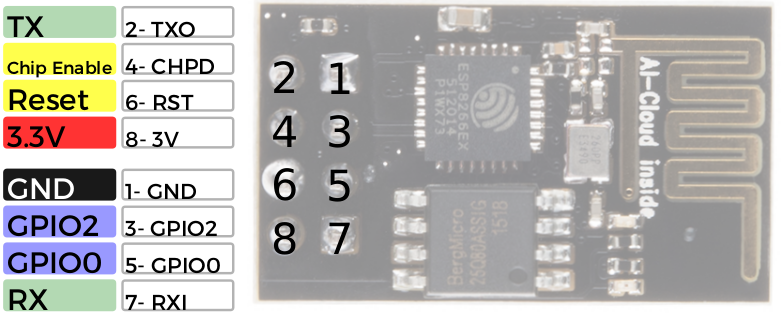
\includegraphics[width=0.9\textwidth]{ESP8266_pinout.png}}
\caption{ESP8266 pinout guide.}
\label{ESP8266_pinout}
\end{figure}
\begin{enumerate}
\item Connect the USB-UART cable to the module : The \texttt{GND} (black) on the pin1, the \texttt{Rx} (yellow) on the \texttt{Tx} and the Tx (Orange) on the Rx of the module. see figure \ref{usb-uart_connection}.
\item Plug the USB end of the cable into a USB port of the computer.
\item Power on and enable the board : Take two female-female cables, connect them to two 3V3 pins, one is the default \texttt{ESP8266\_VCC}, the other can be \texttt{VCC3P3} on the Arduino Extension. see figure \ref{power_on-enable}.
\item Connect the two cables to the \texttt{3.3V} (pin 8) and the \texttt{Chip Enable} (pin 4) of the module. A red led should be on.
\item Pull-down the \texttt{GPIO0} pin of the ESP8266 (pin 5) : take a third cable, connect it to a ground on the board.
\end{enumerate}
\begin{figure}[H]
\makebox[\textwidth][c]{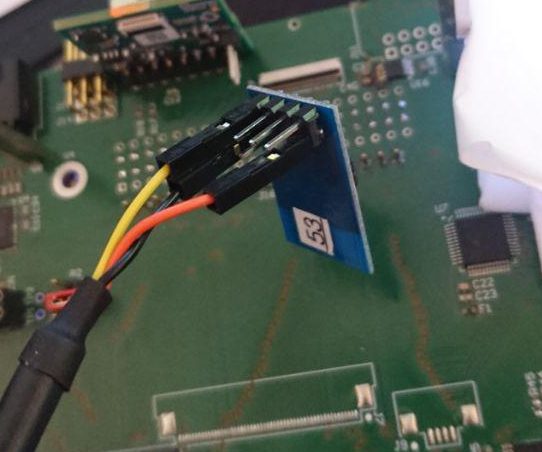
\includegraphics[scale=0.5]{usb-uart_connection.jpg}}
\caption{Connection of the USB-UART cable.}
\label{usb-uart_connection}
\end{figure}
\begin{figure}[H]
\makebox[\textwidth][c]{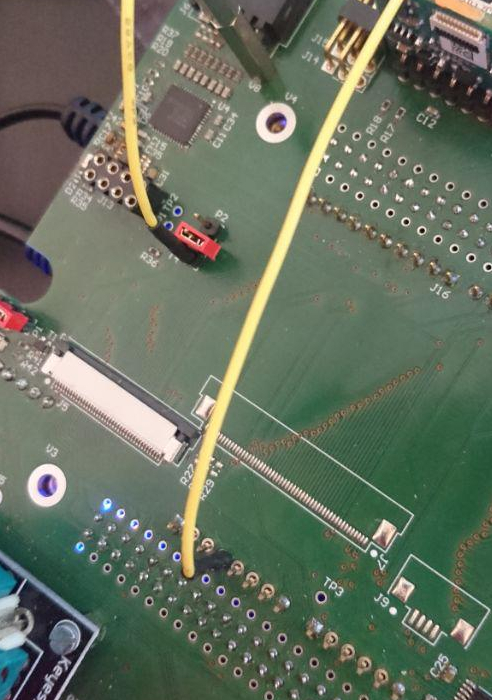
\includegraphics[scale=0.5  ]{power_on-enable.jpg}}
\caption{Connection of the two female-female cables to 3.3 volts sources.}
\label{power_on-enable}
\end{figure}
You should have the following setup :
\begin{figure}[H]
\makebox[\textwidth][c]{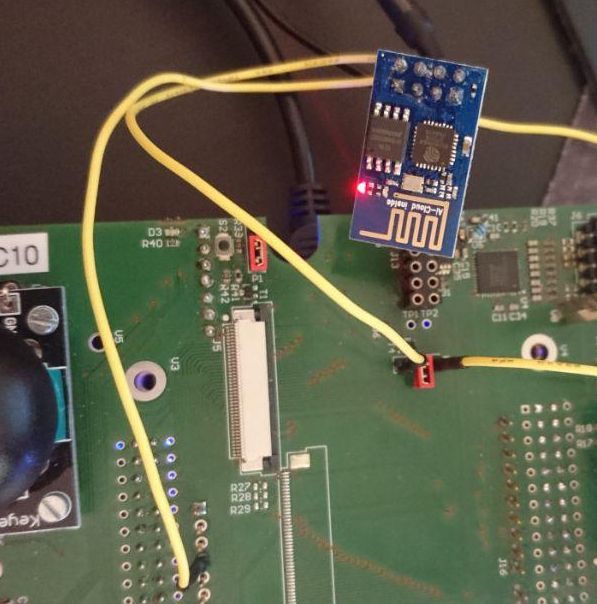
\includegraphics[scale=0.5]{ESP8266_setup.jpg}}
\caption{Complete setup for flashing the module.}
\label{ESP8266_setup}
\end{figure}

Now it is time to upgrade the Firmware. We assume the USB-UART serial cable is identified as \texttt{\textbackslash dev\textbackslash ttyUSB0}.
\begin{enumerate}
\item unzip the archive : \texttt{\$ unzip esptool-master.zip},
\item go to the extrated folder : \texttt{\$ cd esptool-master},
\item run the program the with flash memory parameters already located in the folder : \\
\texttt{\$ ./esptool.py -p /dev/ttyUSB0 write\_flash 0x0000 \textbackslash \\
boot\_v1.7.bin 0x01000 user1.1024.new.2.bin 0x7C000 \textbackslash \\
esp\_init\_data\_default.bin 0x7E000 blank.bin}
\end{enumerate}
You should see the following output on the terminal :
\begin{figure}[H]
\makebox[\textwidth][c]{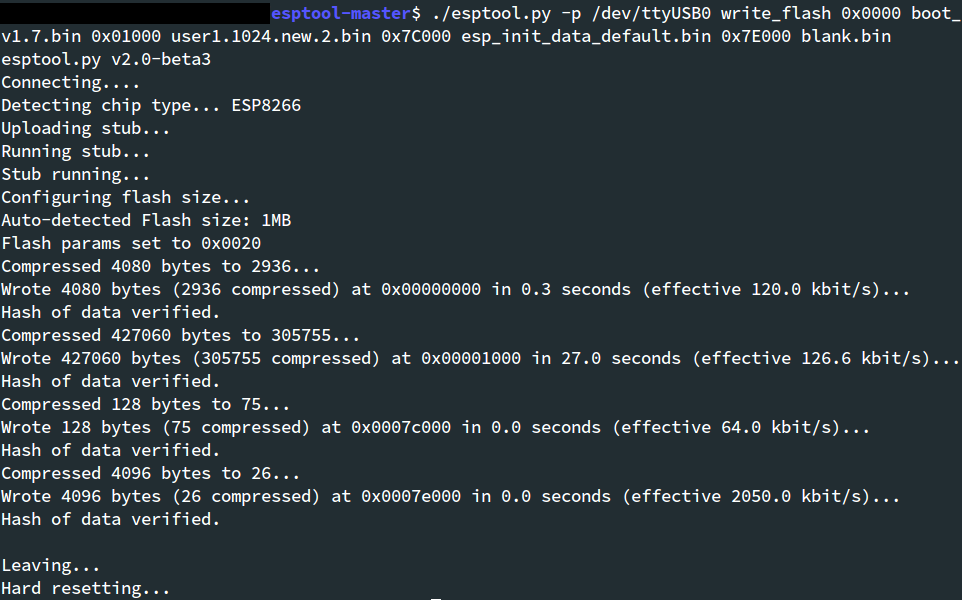
\includegraphics[width=\textwidth]{Flashing_eps8266.png}}
\caption{Output of the flashing program.}
\label{Flashing_eps8266}
\end{figure}
If there is any missing library from Python2, you should install them. In particular, it needs \texttt{pyserial2.7}.
If the program keep trying to connect without managing, check the connectivity and/or try to unplug both 3.3V cables (\texttt{VCC} and \texttt{Chip enable}) and then replug them.

\section{Testing}
Now we want to test if the flash was successful. Unplug the wire to the GPIO0 pin of the module\\
Using your favourite USB-UART communication tool (here we will use PuTTY), open a serial connection with the following settings :
\begin{itemize}
\item Speed (baud) = 115200,
\item Data bits = 8,
\item Stop bits = 1,
\item No Parity or Flow Control.
\end{itemize}
These settings are now default ones stored inside the memory.\\
Now you can try to send any command in the AT commands set.\\
The commands should end by "\textbackslash r\textbackslash n", which can be done by entering '\textasciicircum M' and '\textasciicircum J' (ctrl+'m' and ctr+'j').\\
By default, the module will echo whatever you input on it's Rx line to the Tx, that's why you see what you type. It can be turned off by entering the "ATE0\textbackslash r\textbackslash n" command.\\
\begin{figure}[H]
\makebox[\textwidth][c]{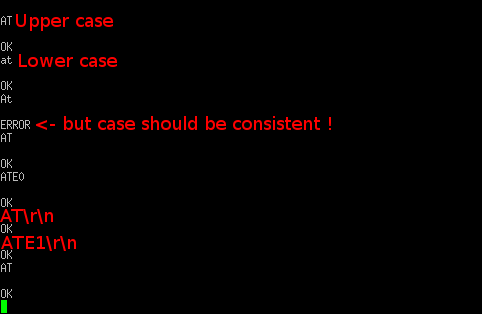
\includegraphics[width=\textwidth]{putty_exemple.png}}
\caption{Exemple of test using PuTTY.}
\label{putty_exemple}
\end{figure}
\end{document}
